\section{Problem Examples}
At present, our system includes seven CTF challenges, with one
disabled due to missing a key file. To give a sense of the style of
problems, and expected interactions with the problems, we will now
outline two different included challenges.

\subsection{Hitcon 2014's rsaha}
todo:ben
\subsection{PlaidCTF 2014's parlor}

\begin{figure}[h!]
\begin{centering}
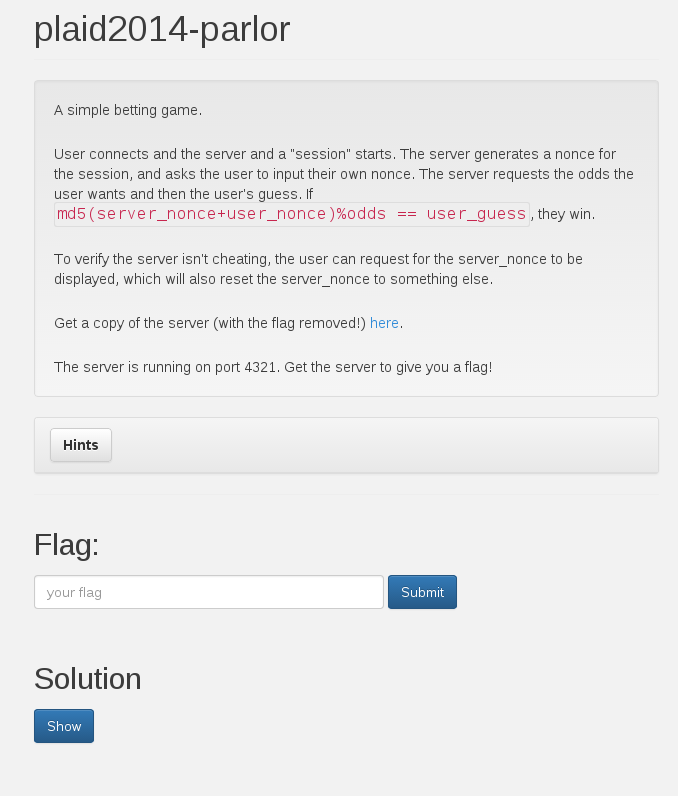
\includegraphics[width=0.5\textwidth]{parlor_page.png}
\caption{Plaid2014 parlor challenge page}
\end{centering}
\label{fig:parlor_page}
\end{figure}

\begin{figure}[h!]
\begin{centering}
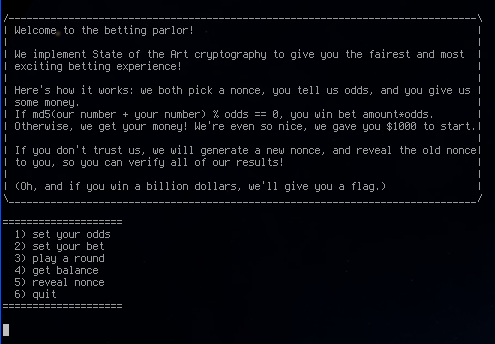
\includegraphics[width=0.5\textwidth]{parlor_interface.png}
\caption{Plaid2014 parlor server text-based interface}
\end{centering}
\label{fig:parlor_interface}
\end{figure}


This challenge is a small server that runs a betting game. The game is
designed around guessing the last digits of a hash, which is
constructed via \texttt{md5(snonce+pnonce)}. The two nonces are from
the server (\texttt{snonce}) and the player
(\texttt{pnonce}). However, the server re-uses the server nonce until
the player asks for it to verify the server did not cheat. This
creates a situation where the server is vulnerable to a
\textit{hash-length extension} attack. When the player submits a
nonce, they get back the lower 100 bits of the resulting md5sum. By
obtaining two sample set of bits from \texttt{md5(snonce+X)} and
\texttt{md5(snonce+X+L)}, the player can brute-force the first 28 bits
of the md5sum and verify by using a hash-length extension attack
tool. From there, they can generate the $L$ value they desire to
always win the bet. After winning a (otherwise statistically
impossible) large number of bets, the server will hand back a 'flag'
as a reward.

This problem represents a very standard CTF problem design; a very
basic contained server (just a single python file) that plays an
ostensibly fair game that cannot be won fairly. Our design makes
integrating problems like this very simple. Filling out the
description and hints is straight forward, while the suggested reading
had to be careful not to only include links to hash-length extension
attacks. The server configuration is mostly handled by the templated
init script that the new problem generation tool will use. The problem
designer needs only fill out two lines of a configuration file (with
the problem name and server binary), and write any description and
solution information they wish to include.

Figure \ref{fig:parlor_page} shows the rendered page generated by our
scripts for this problem. After connecting to the server on the port
specified (via \texttt{nc localhost 4321}) they are presented with the
problem interface as designed by the challenge author (see Figure
\ref{fig:parlor_interface}.) This is a very standard looking CTF
challenge, with a basic text-based server interface.
